\documentclass[]{book}
\usepackage{lmodern}
\usepackage{amssymb,amsmath}
\usepackage{ifxetex,ifluatex}
\usepackage{fixltx2e} % provides \textsubscript
\ifnum 0\ifxetex 1\fi\ifluatex 1\fi=0 % if pdftex
  \usepackage[T1]{fontenc}
  \usepackage[utf8]{inputenc}
\else % if luatex or xelatex
  \ifxetex
    \usepackage{mathspec}
  \else
    \usepackage{fontspec}
  \fi
  \defaultfontfeatures{Ligatures=TeX,Scale=MatchLowercase}
\fi
% use upquote if available, for straight quotes in verbatim environments
\IfFileExists{upquote.sty}{\usepackage{upquote}}{}
% use microtype if available
\IfFileExists{microtype.sty}{%
\usepackage{microtype}
\UseMicrotypeSet[protrusion]{basicmath} % disable protrusion for tt fonts
}{}
\usepackage{hyperref}
\hypersetup{unicode=true,
            pdftitle={Proctor Foundation Data Science Handbook},
            pdfauthor={Contributors (many from UC Berkeley in addition to Proctor): Ben Arnold, Jade Benjamin-Chung, Kunal Mishra, Stephanie Djajadi, Nolan Pokpongkiat},
            pdfborder={0 0 0},
            breaklinks=true}
\urlstyle{same}  % don't use monospace font for urls
\usepackage{natbib}
\bibliographystyle{apalike}
\usepackage{longtable,booktabs}
\usepackage{graphicx,grffile}
\makeatletter
\def\maxwidth{\ifdim\Gin@nat@width>\linewidth\linewidth\else\Gin@nat@width\fi}
\def\maxheight{\ifdim\Gin@nat@height>\textheight\textheight\else\Gin@nat@height\fi}
\makeatother
% Scale images if necessary, so that they will not overflow the page
% margins by default, and it is still possible to overwrite the defaults
% using explicit options in \includegraphics[width, height, ...]{}
\setkeys{Gin}{width=\maxwidth,height=\maxheight,keepaspectratio}
\IfFileExists{parskip.sty}{%
\usepackage{parskip}
}{% else
\setlength{\parindent}{0pt}
\setlength{\parskip}{6pt plus 2pt minus 1pt}
}
\setlength{\emergencystretch}{3em}  % prevent overfull lines
\providecommand{\tightlist}{%
  \setlength{\itemsep}{0pt}\setlength{\parskip}{0pt}}
\setcounter{secnumdepth}{5}
% Redefines (sub)paragraphs to behave more like sections
\ifx\paragraph\undefined\else
\let\oldparagraph\paragraph
\renewcommand{\paragraph}[1]{\oldparagraph{#1}\mbox{}}
\fi
\ifx\subparagraph\undefined\else
\let\oldsubparagraph\subparagraph
\renewcommand{\subparagraph}[1]{\oldsubparagraph{#1}\mbox{}}
\fi

%%% Use protect on footnotes to avoid problems with footnotes in titles
\let\rmarkdownfootnote\footnote%
\def\footnote{\protect\rmarkdownfootnote}

%%% Change title format to be more compact
\usepackage{titling}

% Create subtitle command for use in maketitle
\providecommand{\subtitle}[1]{
  \posttitle{
    \begin{center}\large#1\end{center}
    }
}

\setlength{\droptitle}{-2em}

  \title{Proctor Foundation Data Science Handbook}
    \pretitle{\vspace{\droptitle}\centering\huge}
  \posttitle{\par}
    \author{Contributors (many from UC Berkeley in addition to Proctor): Ben Arnold, Jade Benjamin-Chung, Kunal Mishra, Stephanie Djajadi, Nolan Pokpongkiat}
    \preauthor{\centering\large\emph}
  \postauthor{\par}
      \predate{\centering\large\emph}
  \postdate{\par}
    \date{2019-10-01}

\usepackage{booktabs}

\begin{document}
\maketitle

{
\setcounter{tocdepth}{1}
\tableofcontents
}
\hypertarget{welcome}{%
\chapter*{Welcome!}\label{welcome}}
\addcontentsline{toc}{chapter}{Welcome!}

Welcome to the Francis I. Proctor Foundation at the University of California, San Francisco (\url{https://proctor.ucsf.edu})!

This handbook summarizes some best practices for data science, drawing from our experience at the Francis I. Proctor Foundation and from that of our close colleagues in the Division of Epidemiology and Biostatistics at the University of California, Berkeley (where Prof.~Ben Arnold worked for many years before joining Proctor).

We do not intend this handbook to be a comprehensive guide to data science. Instead, it focuses more on practical, ``how-to'' guidance for conducting data science within epidemiologic research studies. Although many of the ideas of environment-independent, the examples draw from the \href{https://cran.r-project.org/}{R} programming language. For an excellent overview of data science in R, see the book \href{https://r4ds.had.co.nz/}{R for Data Science}.

Much of the material in this handbook evolved from a version of Dr.~Jade Benjamin-Chung's \href{https://github.com/jadebc-berkeley/lab-manual}{lab manual} at the University of California, Berkeley. In addition to the Proctor team, many contributors include current and former students from UC Berkeley.

The last two chapters of the handbook cover our communication strategy and code of conduct for team members who work with Prof.~Ben Arnold, who leads Proctor's Data Coordinating Center. They summarize key pieces of a functional data science team. Although the last two chapters might be of interest to a broader circle, \emph{they are mostly relevant for people working directly with Ben.} Just because they are at the end does not make them less important.

It is a living document that we strive to update regularly. If you would like to contribute, please write Ben (\href{mailto:ben.arnold@ucsf.edu}{\nolinkurl{ben.arnold@ucsf.edu}}) and/or submit a pull request.

The GitHub repository for this handbook is: \url{https://github.com/proctor-ucsf/dcc-handbook}

\hypertarget{intro}{%
\chapter{Introduction: Work Flow and Reproducible Analyses}\label{intro}}

\emph{Contributors: Ben Arnold}

This handbook collates a number of tips to help organize the workflow of epidemiologic data analyses. There are probably a dozen good ways to organize a workflow for reproducible research. This document includes recommendations that arise from our own team's experience through numerous field trials and observational data analyses. The recommendations will not work for everybody or for all applications. But, they work well for most of us most of the time, else we wouldn't put in the time to share them.

Start with two organizing concepts:

\begin{itemize}
\item
  \textbf{Workflow}. Defined here as the process required to draw scientific inference from data collected in the field or lab. I.e., the process by which we take data, and then process it, share it internally, analyze it, and communicate results to the scientific community.
\item
  \textbf{Reproducible research}. A fundamental characteristic of the scientific method is that study findings can be reproduced beyond the original investigators. Data analyses that contribute to scientific research should be described and organized in a way that they could be reproduced by an independent person or research group. A data analysis that is not reproducible violates a core principle of the scientific method.
\end{itemize}

\hypertarget{workflow}{%
\section{Workflow}\label{workflow}}

Broadly speaking, a typical scientific data science work flow involves four steps to transform raw data (e.g., from the field) into summaries that communicate results to the scientific community.

\begin{figure}
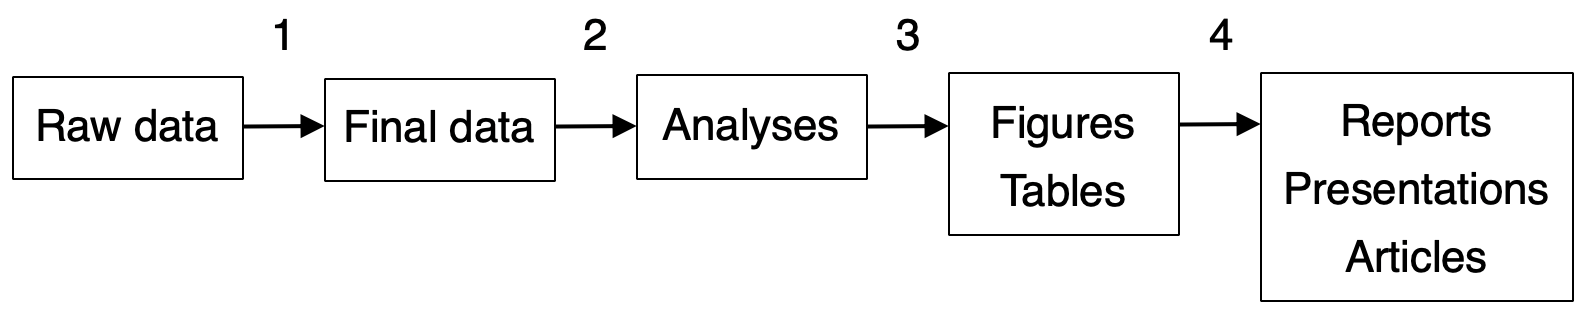
\includegraphics[width=0.75\linewidth]{/Users/benarnold/dcc-handbook/images/workflow} \caption{Overview of the four main steps in a typical data science workflow}\label{fig:fig-workflow}
\end{figure}

When starting a new project, the work flow tends to evolve gradually and by iteration. Data cleaning, data processing, exploratory analyses, back to data cleaning, and so forth. If the work takes place in an unstructured environment with no system to organize files and work flow, it rapidly devolves into into a disorganized mess; analyses become difficult or impossible to replicate and they are anything but scientific. Projects with short deadlines (e.g., proposals, conference abstract submissions, article revisions) are particularly vulnerable to this type of organizational entropy. Putting together a directory and workflow plan from the start helps keep files organized and prevent disorder. Modifications are inevitable -- as long as the system is organized, modifications are usually no problem.

Depending on the project, each step involves a different amount of work. Step 1 is by far the most time consuming, and often the most error-prone. We devote an entire chapter to it below (\protect\hyperlink{datacleaning}{Data cleaning and processing})

\hypertarget{reproducibility}{%
\section{Reproducibility}\label{reproducibility}}

As a guiding directive, this process should be reproducible. If you are not familiar with the concept of reproducible research, start with this manifesto (\href{https://www.nature.com/articles/s41562-016-0021}{Munafo et al.~2017}). For a deeper dive, we highly recommend the recent book from Christensen, Freese, and Miguel (\href{https://www.ucpress.edu/book/9780520296954/transparent-and-reproducible-social-science-research}{2019}). Although it is framed around social science, the ideas apply generally.

\hypertarget{automation}{%
\section{Automation}\label{automation}}

We recommend that the workflow be as automated as possible using a programming language. Automating the workflow in a programming language, and essentially reducing it to text, is advantageous because it makes the process transparent, well documented, easily modified, and amenable to version control; these characteristics lend themselves to reproducible research.

At Proctor, we mostly use R. With the development of \href{https://rstudio.com/}{Rstudio}, \href{https://rmarkdown.rstudio.com/}{R Markdown} and the \href{https://www.tidyverse.org/}{tidyverse} ecosystem (among others), the R language has evolved as much in the past few years as in all previous decades since its inception. This has made the conduct of automated, reproducible research considerably easier than it was 10 years ago.

\textbf{If you have a step in your analysis workflow that involves point-and-click or copy/paste, then STOP, and ask yourself (and your team): } \textbf{\emph{How can I automate this?}}

\hypertarget{workflows}{%
\chapter{Workflows}\label{workflows}}

\emph{Contributors: Ben Arnold}

A data science work flow typically progresses through 4 steps that rarely evolve in a purely linear fashion, but in the end should flow in this direction:

\begin{figure}
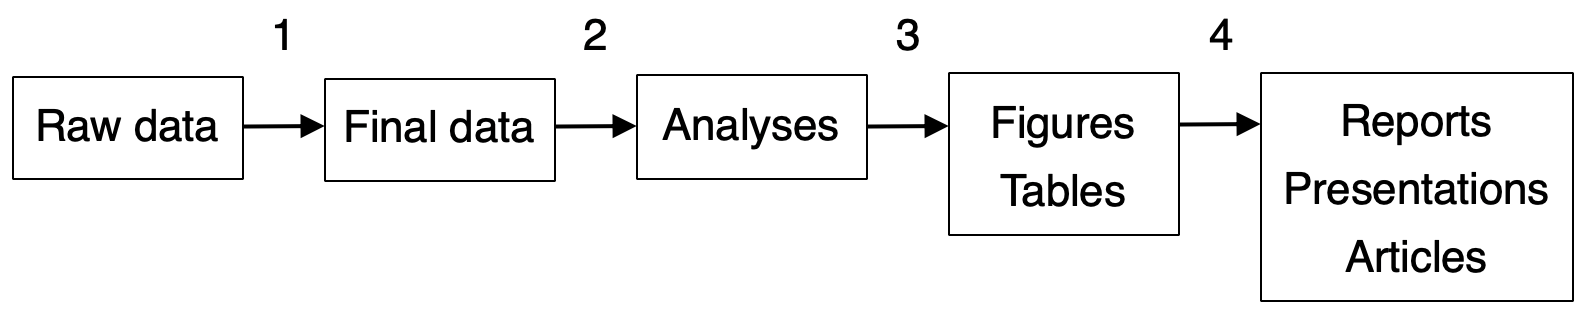
\includegraphics[width=0.75\linewidth]{/Users/benarnold/dcc-handbook/images/workflow} \caption{Overview of the four main steps in a typical data science workflow}\label{fig:fig-workflow2}
\end{figure}

\begin{longtable}[]{@{}clcc@{}}
\caption{\label{tab:workflow} Workflow basics}\tabularnewline
\toprule
\begin{minipage}[b]{0.07\columnwidth}\centering
Steps\strut
\end{minipage} & \begin{minipage}[b]{0.25\columnwidth}\raggedright
Example activities\strut
\end{minipage} & \begin{minipage}[b]{0.28\columnwidth}\centering
\(\Rightarrow\) Inputs\strut
\end{minipage} & \begin{minipage}[b]{0.29\columnwidth}\centering
\(\Rightarrow\) Outputs\strut
\end{minipage}\tabularnewline
\midrule
\endfirsthead
\toprule
\begin{minipage}[b]{0.07\columnwidth}\centering
Steps\strut
\end{minipage} & \begin{minipage}[b]{0.25\columnwidth}\raggedright
Example activities\strut
\end{minipage} & \begin{minipage}[b]{0.28\columnwidth}\centering
\(\Rightarrow\) Inputs\strut
\end{minipage} & \begin{minipage}[b]{0.29\columnwidth}\centering
\(\Rightarrow\) Outputs\strut
\end{minipage}\tabularnewline
\midrule
\endhead
\begin{minipage}[t]{0.07\columnwidth}\centering
1\strut
\end{minipage} & \begin{minipage}[t]{0.25\columnwidth}\raggedright
\textbf{Data cleaning and processing}\strut
\end{minipage} & \begin{minipage}[t]{0.28\columnwidth}\centering
\strut
\end{minipage} & \begin{minipage}[t]{0.29\columnwidth}\centering
\strut
\end{minipage}\tabularnewline
\begin{minipage}[t]{0.07\columnwidth}\centering
.\strut
\end{minipage} & \begin{minipage}[t]{0.25\columnwidth}\raggedright
make a plan for final datasets, fix data entry errors, create derived variables, plan for public replication files\strut
\end{minipage} & \begin{minipage}[t]{0.28\columnwidth}\centering
untouched datasets\strut
\end{minipage} & \begin{minipage}[t]{0.29\columnwidth}\centering
final datasets\strut
\end{minipage}\tabularnewline
\begin{minipage}[t]{0.07\columnwidth}\centering
2-3\strut
\end{minipage} & \begin{minipage}[t]{0.25\columnwidth}\raggedright
\textbf{Analyses}\strut
\end{minipage} & \begin{minipage}[t]{0.28\columnwidth}\centering
\strut
\end{minipage} & \begin{minipage}[t]{0.29\columnwidth}\centering
\strut
\end{minipage}\tabularnewline
\begin{minipage}[t]{0.07\columnwidth}\centering
.\strut
\end{minipage} & \begin{minipage}[t]{0.25\columnwidth}\raggedright
exploratory data analysis, study monitoring, summary statistics, statistical analyses, independent replication of analyses, make figures and tables\strut
\end{minipage} & \begin{minipage}[t]{0.28\columnwidth}\centering
final datasets\strut
\end{minipage} & \begin{minipage}[t]{0.29\columnwidth}\centering
saved results (.rds/.csv), tables (.html,.pdf), figures (.html/.png)\strut
\end{minipage}\tabularnewline
\begin{minipage}[t]{0.07\columnwidth}\centering
4\strut
\end{minipage} & \begin{minipage}[t]{0.25\columnwidth}\raggedright
\textbf{Communication}\strut
\end{minipage} & \begin{minipage}[t]{0.28\columnwidth}\centering
\strut
\end{minipage} & \begin{minipage}[t]{0.29\columnwidth}\centering
\strut
\end{minipage}\tabularnewline
\begin{minipage}[t]{0.07\columnwidth}\centering
.\strut
\end{minipage} & \begin{minipage}[t]{0.25\columnwidth}\raggedright
results synthesis\strut
\end{minipage} & \begin{minipage}[t]{0.28\columnwidth}\centering
saved results, figures, tables\strut
\end{minipage} & \begin{minipage}[t]{0.29\columnwidth}\centering
monitoring reports, presentations, scientific articles\strut
\end{minipage}\tabularnewline
\bottomrule
\end{longtable}

In many modern data science workflows, steps 2-4 can be accomplished in a single R notebook or Jupyter notebook: the statistical analysis, creation of figures and tables, and creation of reports.

However, it is still useful to think of the distinct stages in many cases. For example, a single statistical analysis might contribute to a DSMC report, a scientific conference presentation, and a scientific article. In this example, each piece of scientific communication would take the same input (stored analysis results as .csv/.rds) and then proceed along slightly different downstream workflows.

It would be more error prone to replicate the same statistical analysis in three parallel downstream work flows. This illustrates a key idea that holds more generally:

\begin{longtable}[]{@{}l@{}}
\toprule
\endhead
\textbf{Key idea for workflows:} Whenever possible, avoid repeating the same data processing or statistical analysis in separate streams. \emph{Key data processing and analyses should be done once}.\tabularnewline
\bottomrule
\end{longtable}

\hypertarget{directory-structure-and-code-repositories}{%
\chapter{Directory Structure and Code Repositories}\label{directory-structure-and-code-repositories}}

\emph{Contributors: Kunal Mishra, Jade Benjamin-Chung, Ben Arnold}

The backbone of your project workflow is the file directory so it makes sense to spend time organizing the directory. Note that \texttt{directory} is the technical term for the system used to organize individual files. Most non-UNIX environments use a folder analogy, and directory and folder can be used interchangeably in a lot of cases. A well organized directory will make everything that follows much easier. Just like a well designed kitchen is essential to enjoy cooking (and avoid clutter), a well designed directory helps you enjoy working and stay organized in a complex project with literally thousands of related files. Just like a disorganized kitchen (``now where did I put that spatula?'') a disorganized project directory creates confusion, lost time, stress, and mistakes.

Another huge advantage of maintaining a regular/predictable directory structure within a project and across projects is that it makes it more intuitive. When a directory is intuitive, it is easier to work collaboratively across a larger team; everybody can predict (at least approximately) where files should be.

Nested within your directory will be a \texttt{code\ repository}. Sometimes we find it useful to manage the code repository using version control, such as git/GitHub.

Other chapters will discuss \protect\hyperlink{codingpractices}{coding practices}, \protect\hyperlink{datamanagement}{data management}, and \protect\hyperlink{github}{GitHub/version control} that will build from the material here.

Carrying the kitchen analogy further: here, we are designing the kitchen. Then, we'll discuss approaches for how to cook in the kitchen that we designed/built.

\hypertarget{small-and-large-projects}{%
\section{Small and large projects}\label{small-and-large-projects}}

Our experience is that the overwhelming majority of projects come in two sizes: small and large. We recommend setting up your directory structure depending on how large you expect the project to be. Sometimes, small projects evolve into large projects, but only occasionally. A small project is something like a single data analysis with a single published article in mind. A large project is an epidemiologic field study, where there are multiple different types of data and different types of analyses (e.g., sample size calculations, survey data, biospecimens, substudies, etc.).

\begin{center}\rule{0.5\linewidth}{\linethickness}\end{center}

\textbf{Small project:} There is essentially one dataset and a single, coherent analysis. For example, a simulation study or a methodology study that will lead to a single article.

\textbf{Large project:} A field study that includes multiple activities, each of which generates data files. Multiple analyses are envisioned, leading to multiple scientific articles.

\begin{center}\rule{0.5\linewidth}{\linethickness}\end{center}

Large projects are more common and more complicated. Most of this chapter focuses on large project organization (small projects can be thought of as essentially one piece of a large project).

\hypertarget{directory-structure}{%
\section{Directory Structure}\label{directory-structure}}

In the example below, we follow a basic directory naming convention that makes working in UNIX and typing directory statements in programs much easier:

\begin{itemize}
\tightlist
\item
  \textbf{short names}
\item
  \textbf{no spaces in the names} (not essential but a personal preference. Can use \texttt{\_} or \texttt{-} instead)
\item
  \textbf{lower case} (not essential, again, personal preferences vary!)
\end{itemize}

For example, Ben completed a study in Tamil Nadu, India during his dissertation to study the effect of improvements in water supply and sanitation on child health. Instead of naming the directory \texttt{Tamil\ Nadu} or \texttt{Tamil\ Nadu\ WASH\ Study}, he used \texttt{trichy} instead (a colloquial name for the city near the study, Tiruchirappalli), which was much easier to type in the terminal and in directory statements. A short name helps make directory references easier while programming.

\hypertarget{first-level-data-and-analyses}{%
\subsection{First level: data and analyses}\label{first-level-data-and-analyses}}

\begin{figure}
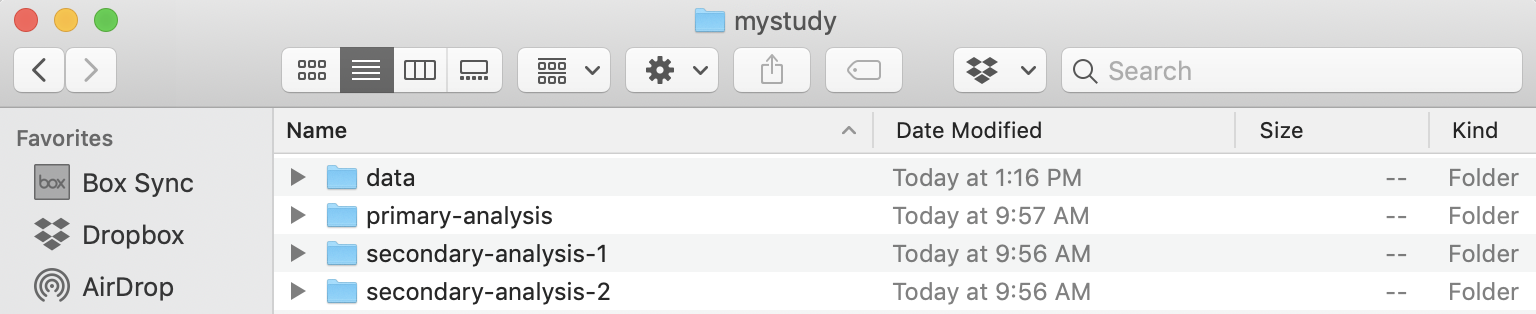
\includegraphics[width=0.75\linewidth]{/Users/benarnold/dcc-handbook/images/mystudy-dir-fig1} \caption{Example directory for `mystudy`}\label{fig:dir-fig1}
\end{figure}

Start by dividing a project into major activities. In the example abpve, the project is named \texttt{mystudy}. There is a \texttt{data} subdirectory (more in a sec), and then three major activities, each corresponding to a separate analysis: \texttt{primary-analysis},\texttt{secondary-analysis-1}, and \texttt{secondary-analysis-2}. In a real project, the names could be more informative, such as ``trachoma-qpcr''. Also, a real project might also include many additional subdirectories related to administrative and logistics activities that do not relate to data science, such as irb, travel, contracts, budget, survey forms, etc.).

Dividing files into major activities helps keep things organized for really big projects. In a multi-site study, consider including a directory for each site before splitting files into major activities. Ideally, analyses will not span major activity subdirectories in a project folder, but sometimes you can't predict/avoid that from happening.

\hypertarget{second-level-data}{%
\subsection{Second level: data}\label{second-level-data}}

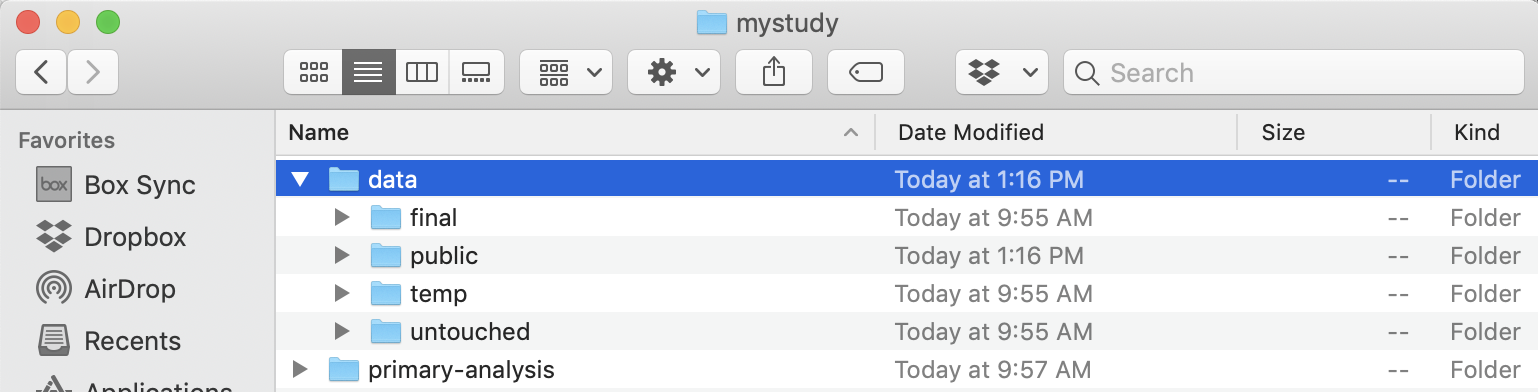
\includegraphics[width=0.75\linewidth]{/Users/benarnold/dcc-handbook/images/mystudy-dir-fig2}

Each project will include a \texttt{data} directory. We recommend organizing it into 3 parts: \texttt{untouched}, \texttt{temp}, and \texttt{final}. Often, it is useful to include a fourth subdirectory called \texttt{public} for sharing public versions of datasets.

The \texttt{untouched} directory includes all untouched datasets that are used for the study. Once saved in the directory never touch them; you will read them into the work flow, but \textbf{never, ever save over them}. If the study has repeated extracts from rolling data collection or electronic health records, consider subdirectories within \texttt{untouched} that are indexed by date.

The \texttt{temp} directory (optional, not essential) includes temporary files that you might generate during the data management process. This is mainly a space for experimentation. As a rule, never save anything in the temp directory that you cannot delete. Regularly delete files in the temp directory to save disk space.

The \texttt{final} directory includes final datasets for the activity. Final datasets are de-identified and require no further processing; they are clean and ready for analysis. They should be accompanied by meta-data, which at minimum includes the data's provenance (i.e., how it was created) and what it includes (i.e., level of the data, plus variable coding/labels/descriptions). Clean/final datasets generated by one analysis might be reused in another.

\hypertarget{second-level-analysis}{%
\subsection{Second level: analysis}\label{second-level-analysis}}

We recommend maintaining a separate subdirectory for each major analysis in a project. In this example, there are three with not-very-creative names from the view of trial: \texttt{primary-analysis}, \texttt{secondary-analysis-1}, \texttt{secondary-analysis-2}.

Think of each analysis as the scope of all of the work for a single, published paper. We recommend dividing the analysis project into a space for computational notebooks / scripts (i.e., a \texttt{code\ repository}), and a second for their output. The reason for the split is to make it easier to use version control (should you choose) for the code. Version control like \texttt{git} and \texttt{GitHub} (see the \protect\hyperlink{GitHub}{Chapter on GitHub}) works well for text files but isn't really designed for binary files such as images (.png), datasets (.rds), or PDF files (.pdf). It is certainly possible to use git with those file types, but since git makes a new copy of the file every time it is changed the git repo can get horribly bloated and takes up too much space on disk. Consolidating the output into a separate directory makes it more obvious that it isn't under version control. In this example, there are separate parts for code (\texttt{R}) and output (\texttt{output}). Output could include figures, tables, or saved analysis results stored as data files (.rds or .csv). Another conventional name for the code repository is \texttt{src} as an alternative to \texttt{R} if you use other languages.

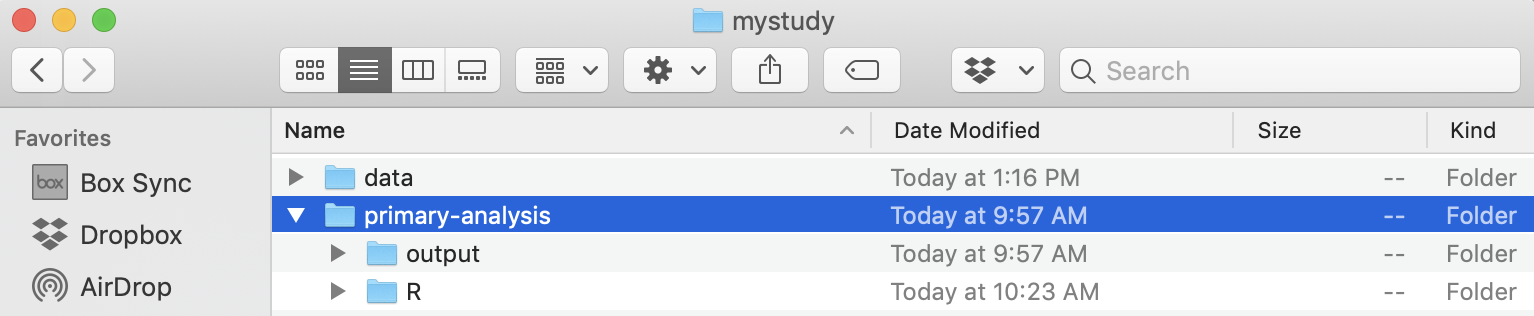
\includegraphics[width=0.75\linewidth]{/Users/benarnold/dcc-handbook/images/mystudy-dir-fig3}

\begin{center}\rule{0.5\linewidth}{\linethickness}\end{center}

\emph{Interdependence between analyses}: Sometimes a result from an analysis might be a cleaned dataset that could feed into future, distinct analyses. This is quite common, for example, in large trials where a set of baseline characteristics might be used in multiple separate papers for different endpoints, either for assessing balance of the trial population or subgroups, or used as adjustment covariates in additional analyses of the trial. In this case, the cleaned dataset would be written to the \texttt{data/final} directory and is thus available for future use.

\begin{center}\rule{0.5\linewidth}{\linethickness}\end{center}

\hypertarget{code-repositories}{%
\section{Code Repositories}\label{code-repositories}}

Maintain a separate code repository for each major analysis activity (last section).

We recommend the following structure for a code repository:

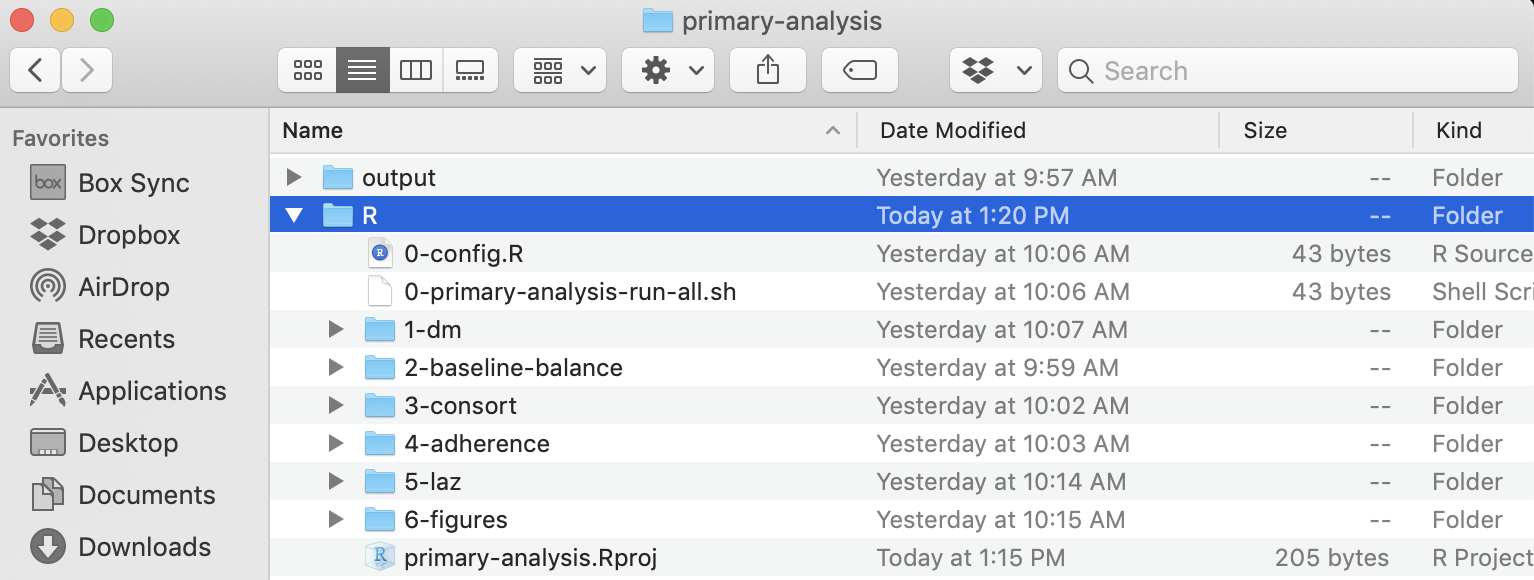
\includegraphics[width=0.75\linewidth]{/Users/benarnold/dcc-handbook/images/mystudy-dir-fig4}

With subdirectories that generally look like this:

\begin{verbatim}
.gitignore
primary-analysis.Rproj
0-config.R
0-primary-analysis-run-all.sh
1-dm /
    0-dm-run-all.sh
    1-format-enrollment-data.R
    2-format-adherence-data.R
    3-format-LAZ-measurements.R
2-baseline-balance /
    0-baseline-balance-run-all.sh
    ...
3-consort /
    0-consort-run-all.sh
    ...
4-adherence /
    0-adherence-run-all.sh
    ...
5-laz /
    0-laz-run-all.sh
    1-laz-unadjusted-analysis.R
    2-laz-adjusted-analysis.R
6-figures / 
    0-figures-run-all.sh
    Fig1-consort.Rmd
    Fig2-adherence.Rmd
    Fig3-laz.Rmd
\end{verbatim}

Note \texttt{dm} is shorthand for ``data management.'' You can call the data management directory anything you want, but just ensure that you have one. This helps ensure work conducted in step 1 of your workflow stays upstream from all analyses (see \protect\hyperlink{workflows}{Chapter on workflows}). Also note that in this example, all of the scripts are \texttt{.R} files. Increasingly, we use R Markdown notebooks \texttt{.Rmd} instead of / in addition to R files.

For brevity, we haven't expanded every directory, but you can glean some important takeaways from what you \emph{do} see.

\hypertarget{rproj-files}{%
\subsection{\texorpdfstring{\texttt{.Rproj} files}{.Rproj files}}\label{rproj-files}}

An ``R Project'' can be created within RStudio by going to \texttt{File\ \textgreater{}\textgreater{}\ New\ Project}. Depending on where you are with your research, choose the most appropriate option. This will save preferences, working directories, and even the results of running code/data (though we recommend starting from scratch each time you open your project, in general). Then, ensure that whenever you are working on that specific research project, you open your created project to enable the full utility of \texttt{.Rproj} files. This also automatically sets the directory to the top level of the project.

\hypertarget{configuration-config-file}{%
\subsection{Configuration (`config') File}\label{configuration-config-file}}

This is the single most important file for your project. It will be responsible for a variety of common tasks, declare global variables, load functions, declare paths, and more. \emph{Every other file in the project} will begin with \texttt{source("0-config")}, and its role is to reduce redundancy and create an abstraction layer that allows you to make changes in one place (\texttt{0-config.R}) rather than 5 different files. To this end, paths that will be referenced in multiple scripts (e.g., a \texttt{clean\_data\_path}) can be declared in \texttt{0-config.R} and simply referred to by its variable name in scripts. If you ever want to change things, rename them, or even switch from a downsample to the full data, all you would then to need to do is modify the path in one place and the change will automatically update throughout your project. See the example config file for more details. The paths defined in the \texttt{0-config.R} file assume that users have opened the \texttt{.Rproj} file, which sets the directory to the top level of the project.

\hypertarget{order-files-and-subdirectories}{%
\subsection{Order Files and Subdirectories}\label{order-files-and-subdirectories}}

This makes the jumble of alphabetized filenames much more coherent and places similar code and files next to one another. Although sometimes there is not a linear progression from 1 to 2 to 3, in general the structure helps reflect how data flows from start to finish and allows us to easily map a script to its output (i.e. \texttt{primary-analysis/R/5-laz/1-laz-unadjusted-analysis.R} =\textgreater{} \texttt{primary-analysis/output/5-laz/1-laz-unadjusted-analysis.RDS}). That is, the code repository and the output are approximately mirrored. If you take nothing else away from this guide, this is the single most helpful suggestion to make your workflow more coherent. Often the particular order of files will be in flux until an analysis is close to completion. At that time it is important to review file order and naming and reproduce everything prior to drafting a manuscript.

In the \texttt{6-figures} subdirectory, each RMarkdown file (computational notebook) is linked to a specific figure in a hypothetical manuscript. This makes it easier to link specific notebooks in figure legends, and to see which file creates each figure.

\hypertarget{use-bash-scripts-to-ensure-reproducibility}{%
\subsection{Use Bash scripts to ensure reproducibility}\label{use-bash-scripts-to-ensure-reproducibility}}

Bash scripts are useful components of a reproducible workflow. At many of the directory levels (i.e.~in \texttt{5-laz}), there is a bash script that runs each of the analysis scripts. This is exceptionally useful when data ``upstream'' changes -- you simply run the bash script. See the \protect\hyperlink{unix}{UNIX Chapter} for further details.

\hypertarget{alternative-approach-for-code-repos}{%
\subsection{Alternative approach for code repos}\label{alternative-approach-for-code-repos}}

Another approach for organizing your code repository is to name all of your scripts according to the final figure or table that they generate for a particular article. In our experience, this \emph{only} works for small projects, with a single set of coherent analyses. Here, you might have an alternative structure such as:

\begin{verbatim}
.gitignore
primary-analysis.Rproj
0-config.R
0-primary-analysis-run-all.sh
1-dm /
    0-dm-run-all.sh
    1-format-enrollment-data.R
    2-format-adherence-data.R
    3-format-LAZ-measurements.R
Fig1-consort.Rmd
Fig2-adherence.Rmd
Fig3-1-laz-analysis.Rmd
Fig3-2-laz-make-figure.Rmd
\end{verbatim}

There is still a need for a separate data management directory (e.g., \texttt{dm}) to ensure that workflow is upstream from the analysis (more below in \protect\hyperlink{unix}{chapter on UNIX}), but then scripts are all together with clear labels. If a figure requires two stages to the analysis, then you can name them sequentially, such as \texttt{Fig3-1-laz-analysis.Rmd}, \texttt{Fig3-2-laz-make-figure.Rmd}. There is no way to divine how all of the analyses will neatly fit into files that correspond to separate figures. Instead, they will converge on these file names through the writing process, often through comsolidation or recombination.

One example of a small repo is here:
\url{https://github.com/ben-arnold/enterics-seroepi}

\hypertarget{codingpractices}{%
\chapter{Coding Practices}\label{codingpractices}}

TBD

\hypertarget{codingstyle}{%
\chapter{Coding Style}\label{codingstyle}}

TBD

\hypertarget{datamanagement}{%
\chapter{Data Management}\label{datamanagement}}

TBD

\hypertarget{github}{%
\chapter{GitHub and Version Control}\label{github}}

TBD

\hypertarget{bigdata}{%
\chapter{Working with Big Data}\label{bigdata}}

TBD

\hypertarget{unix}{%
\chapter{UNIX Commands}\label{unix}}

TBD

\hypertarget{commcoord}{%
\chapter{Communication and Coordination}\label{commcoord}}

\emph{Contributors: Jade Benjamin-Chung, Ben Arnold}

\textbf{These communications guidelines are evolving as we increasingly adopt Slack, but here some general principles if you work closely with Ben.}

\hypertarget{slack}{%
\section{Slack}\label{slack}}

\begin{itemize}
\item
  If you work with Ben but are not a member of Ben's Slack workspace then ask him to invite you!
\item
  Use Slack for scheduling, coding related questions, quick check ins, etc. If your Slack message exceeds 200 words, it might be time to use email.
\item
  Use channels instead of direct messages unless you need to discuss something private.
\item
  Include tags on your message (e.g., \texttt{@Ben}) when you want to ensure that a person sees the message. Ben doesn't regularly read messages where he isn't tagged.
\item
  Please make an effort to respond to messages that message you (e.g., \texttt{@Ben}) as quickly as possible and always within 24 hours, unless of course you are on vacation!
\item
  If you are unusually busy (e.g., taking MCAT/GRE, taking many exams) or on vacation please alert the team in advance so we can expect you not to respond at all / as quickly as usual and also \href{https://get.slack.help/hc/en-us/articles/201864558-Set-your-Slack-status-and-availability}{set your status in Slack} (e.g., it could say ``On vacation'') so we know not to expect to see you online.
\item
  Please thread messages in Slack as much as possible.
\end{itemize}

\hypertarget{email}{%
\section{Email}\label{email}}

\begin{itemize}
\tightlist
\item
  Use email for longer messages (\textgreater{}200 words) or messages that merit preservation.
\item
  Generally, strive to respond within 24 hours. If you are unusually busy or on vacation please alert the team in advance so we can expect you not to respond at all / as quickly as usual.
\end{itemize}

\hypertarget{trello}{%
\section{Trello}\label{trello}}

\begin{itemize}
\tightlist
\item
  Ben manages projects and teams using a \href{https://www.atlassian.com/agile/kanban/boards}{kanban board approach} in \href{https://www.trello.com}{Trello}.
\item
  You and/or Ben will add new cards within our team's Trello boards and assign them to team members.
\item
  Each card represents a discrete chunk of work.
\item
  Cards higher in a list are higher priority.
\item
  Strive to complete the tasks in your card by the card's due date. Talk to Ben about deadlines -- we can always manage the calendar!
\item
  Use checklists to break down a task into smaller chunks. Usually, you can do this yourself (but ask Ben if you ever want input).
\item
  Move cards to the ``DONE'' list on a board when they are done.
\end{itemize}

\hypertarget{google-drive}{%
\section{Google Drive}\label{google-drive}}

\begin{itemize}
\tightlist
\item
  We mostly use Google Drive to create shared documents with longer descriptions of tasks. These documents are linked to Trello cards. Ben often shares these docs with a whole project team since tasks are overlapping, and even if a task is assigned to one person, others may have valuable insights.
\item
  Please invite both of Ben's email addresses to any documents you create (\href{mailto:bfarnold@gmail.com}{\nolinkurl{bfarnold@gmail.com}}, \href{mailto:ben.arnold@ucsf.edu}{\nolinkurl{ben.arnold@ucsf.edu}}).
\end{itemize}

\hypertarget{calendar-meetings}{%
\section{Calendar / Meetings}\label{calendar-meetings}}

\begin{itemize}
\tightlist
\item
  Ben will schedule most meetings through the calendar.
\item
  Our meetings start on the hour.
\item
  If you are going to be late, please send a message in our Slack channel.
\item
  If you are regularly not able to come on the hour, notify the team and we might choose the modify the agenda order or the start time.
\item
  Add hoc meetings are welcome. If Ben's office door is open, come in!
\end{itemize}

\hypertarget{code-of-conduct}{%
\chapter{Code of conduct}\label{code-of-conduct}}

\emph{Contributors: Jade Benjamin-Chung, Ben Arnold}

\hypertarget{group-culture}{%
\section{Group culture}\label{group-culture}}

We strive to work in an environment that is collaborative, supportive, open, and free from discrimination and harassment, per University policies.

We encourage students / staff of all experience levels to respectfully share their honest opinions and ideas on any topic. Our group has thrived upon such respectful honest input from team members over the years, and this document is a product of years of student and staff input (and even debate) that has gradually improved our productivity and overall quality of our work.

If Ben is your PI, be forewarned that he tends to batch his email communication (\textasciitilde{}30 mins in the morning and afternoon, 15 mins mid-day), and doesn't tend to answer Slack or email during evenings or weekends. If you need to reach him urgently then give him a call or text on his mobile.

\hypertarget{protecting-human-subjects}{%
\section{Protecting human subjects}\label{protecting-human-subjects}}

All lab members must complete \href{https://irb.ucsf.edu/citi-human-subjects-training}{CITI Human Subjects Training} and share their certificate with Ben. We will will add team members to relevant Institutional Review Board protocols to ensure they have permission to work with identifiable datasets.

One of the most relevant aspects of protecting human subjects in our work in the Data Coordinating Center is maintaining confidentiality and data privacy. For students supporting our data science efforts, in practice this means:

\begin{itemize}
\tightlist
\item
  If you are using a virtual computer (e.g., Google Cloud, AWS, Optum), never save the data in that system to your personal computer or any other computer without prior permission.
\item
  Do not share data with anyone without first obtaining permission, including to other members of the Proctor Foundation, who might not be on the same IRB protocol as you (check with Ben or the relevant PI first).
\item
  \textbf{NEVER} push a dataset into the public domain (e.g., GitHub, OSF) without first checking with Ben to ensure that it is appropriately de-identified and we have approval from the sponsor and/or human subjects review board to do so.
\end{itemize}

Remember, data that looks like it does not contain identifiers to you might still be classified as data that requires special protection by our IRB or under HIPAA, so always proceed with caution and ask for help if you have any concerns about how to maintain study participant confidentiality. For example, the combination of age, sex, and geographic location of the individual's town or neighborhood is typically considered identifiable.

\hypertarget{authorship}{%
\section{Authorship}\label{authorship}}

We adhere to the \href{http://www.icmje.org/recommendations/browse/roles-and-responsibilities/defining-the-role-of-authors-and-contributors.html}{ICMJE Definition of authorship} and are happy for team members who meet the definition of authorship to be included as co-authors on scientific manuscripts.

\hypertarget{work-hours}{%
\section{Work hours}\label{work-hours}}

Please follow the Proctor Foundation's employee guidelines for work hours, and discuss the specifics with your PI. If Ben is your PI, then work with him on your schedule to ensure we have overlap in the office and that you are around at key times for group meetings, etc.

\hypertarget{resources}{%
\chapter{Additional Resources}\label{resources}}

TBD

\bibliography{book.bib,packages.bib}


\end{document}
